\chapter{СИСТЕМИЙН ЗОХИОМЖ}

\section{Ерөнхий архитектур}

Системийн ерөнхий архитектурыг Зураг~\ref{fig:architecture}--д үзүүлэв. Архитектур нь дөрвөн үндсэн давхаргатай: Chrome extension-д суурилсан хэрэглэгчийн оролтын давхарга, хэлний загвар болон хариултын урсгалыг удирдах AI сервер, SISI API-г MCP хэлбэрт оруулсан локал интеграцын давхарга, SISI, багшийн портал, цаашдын бусад MCP үйлчилгээ зэрэг гаднын системүүд.

\begin{figure}[H]
  \centering
  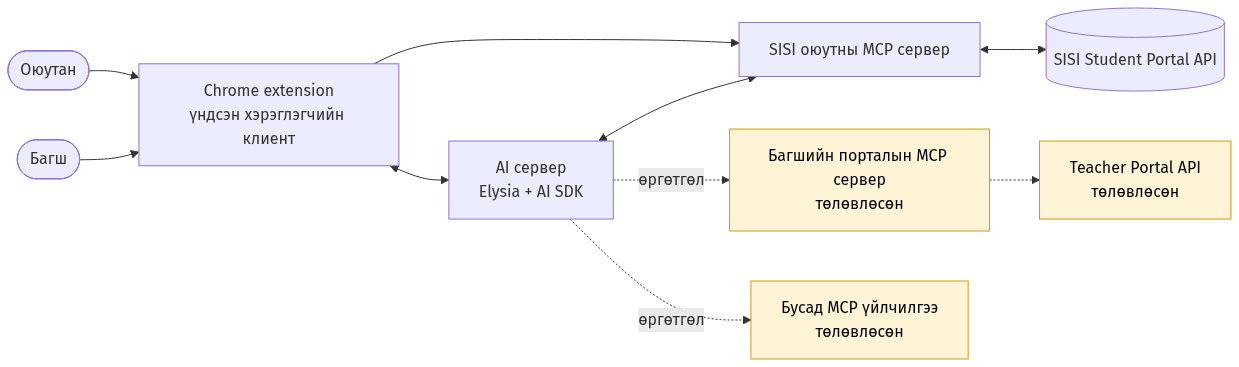
\includegraphics[width=\textwidth]{assets/diagrams/architecture.png}
  \caption{SISi системийн ухаалаг агентын өндөр түвшний архитектур}
  \label{fig:architecture}
\end{figure}

Энэхүү архитектурын гол давуу тал нь Chrome extension, AI сервер, порталын интеграцын давхаргуудыг тусгаарлаж өгсөнд оршино. Ингэснээр хэрэглэгчийн клиент, загвар, MCP серверүүд, read-only болон mutation үйлдлийг бие даан хөгжүүлэх боломж бүрдэнь.

\section{Модулийн зохиомж}

Одоогийн кодын сан дээрх хэрэгжилтийг модульчлан авч үзвэл Хүснэгт~\ref{tab:modules} дахь бүтэцтэй байна.

\begin{table}[H]
  \centering
  \caption{Одоогийн төслийн модулиуд}
  \label{tab:modules}
  \begin{tabularx}{\textwidth}{>{\raggedright\arraybackslash}p{3.4cm} >{\raggedright\arraybackslash}X}
    \toprule
    Модуль & Үүрэг \\
    \midrule
    \texttt{apps/web} & Туршилтын зориулалттай интерфейсийн суурь. Одоогийн зорилтот хэрэглээний үндсэн клиент биш боловч прототип туршихад ашиглагдаж болно. \\
    \texttt{apps/server} & Elysia дээрх AI сервер. Хэлний загвар, message урсгал, цаашдын MCP tool orchestration-ийг удирдах төв давхарга. \\
    \texttt{packages/mcp} & Локал MCP сервер. SISI API-тай холбогдож overview, schedule, academic, financial, notifications, student resources, top menus, e-journal зэрэг хэрэгслийг өгнө. \\
    \texttt{apps/extension} & Chrome extension-ийн үндсэн клиент. Порталын орчноос access token авч, хэрэглэгчийг дахин нэвтрүүлэхгүй session bootstrap хийх зорилготой. \\
    \texttt{packages/db} & Ирээдүйн лог, аудит, үнэлгээний өгөгдөл, mutation үйлдлийн мөрдөх боломжийг хадгалах давхарга. \\
    \bottomrule
  \end{tabularx}
\end{table}

\section{Сесс болон өгөгдлийн урсгал}

SISI API-д хандахын тулд хэрэглэгчийн хүчинтэй сесс шаардлагатай. Иймээс локал MCP сервер нь session register, refresh, clear гэсэн тусдаа endpoint-уудтай бөгөөд эхлээд хэрэглэгчийн сессийг баталгаажуулж байж дараагийн tool call-уудыг зөвшөөрдөг. Энэхүү урсгалыг Зураг~\ref{fig:session-flow}--д үзүүлэв.

\begin{figure}[H]
  \centering
  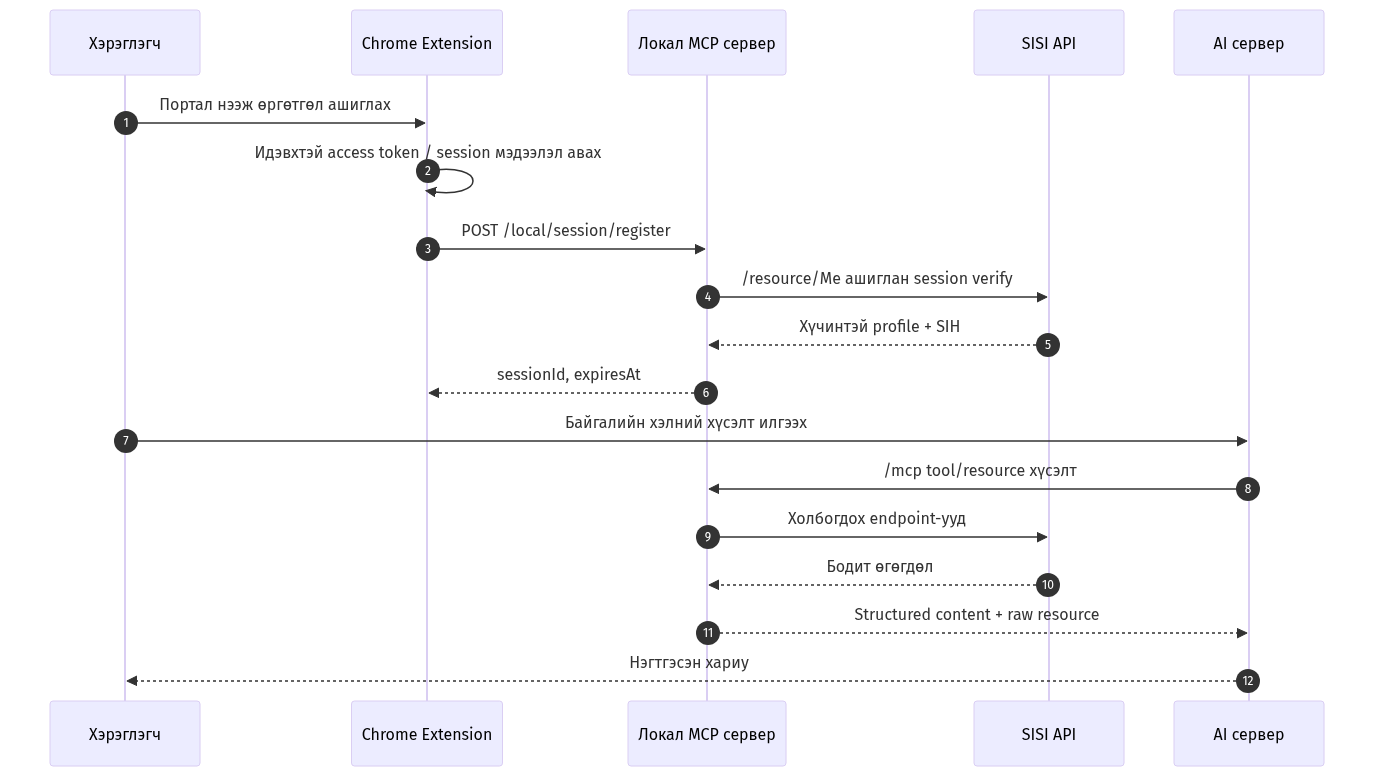
\includegraphics[width=\textwidth]{assets/diagrams/session-bootstrap.png}
  \caption{SISI сесс баталгаажуулалт ба MCP ашиглалтын урсгал}
  \label{fig:session-flow}
\end{figure}

Энэ шийдэл нь порталын access token болон cookie-г AI загварт шууд ил гаргахгүй, session idle TTL ашиглан локал сессийн насыг хязгаарлаж, хөтөчийн origin allowlist-аар зөвшөөрөгдсөн эх сурвалжаас л сесс бүртгэх боломжтой, мөн ижил механизмыг цаашдын багшийн портал болон бусад MCP интеграцын permission flow-д өргөтгөх боломжтой зэрэг шалтгаанаар хэрэгтэй.

\section{Домэйн төвтэй MCP загвар}

SISi системийн ухаалаг агентын интеграцын давхаргыг нэг том endpoint-оор бус, домэйнүүдээр салгасан. Одоогийн байдлаар дараах read-only домэйнүүд тодорхойлогдоод байна: Overview-д оюутны үндсэн мэдээлэл, нүүр хуудасны өгөгдөл, идэвхтэй хичээлүүд, Schedule-д хичээлийн болон шалгалтын хуваарь, Academic-д GPA, transcript, curriculum, request status, Financial-д төлбөр, үлдэгдэл, банкны мэдээлэл, Notifications-д аппын мэдэгдэл болон news, Student resources-д гарын авлага, баримт бичиг, картын мэдээлэл, Top menus/e-journal-д сонголтын туслах өгөгдөл, дүнгийн зарим нэгжүүд багтдаг.

Ийнхүү домэйнээр хуваасан нь дараа нь AI загварт ``ямар зорилгод ямар хэрэгсэл ашиглах вэ'' гэдгийг тогтмол дүрэмтэй болгоход тустай.

\section{Ирээдүйн өргөтгөлийн загвар}

Эцсийн зорилтот системд календарь, баримт бичиг, экспорт, мэдэгдэл зэрэг төрөл бүрийн гаднын үйлчилгээг MCP-ээр холбох ерөнхий MCP өргөтгөлүүд, багшийн API-г MCP хэлбэрт оруулж дүн оруулах зэрэг mutation workflow-г аюулгүй болгох багшийн порталын интеграц, мөн багш олон оюутны дүнг Excel файлаас уншуулан системд оруулах ажлыг хөнгөвчлөх Excel-д суурилсан ажиллагаа зэрэг өргөтгөлүүдийг шат дараатайгаар нэмэхээр төлөвлөж байна.

Эдгээрийг AI серверт хатуу кодлохын оронд тусдаа MCP server буюу MCP-compatible tool layer болгон оруулах нь архитектурын хувьд илүү оновчтой. Ингэснээр SISi системийн ухаалаг агент нь тодорхой нэг үйлчилгээтэй хэт холбогдсон хэрэгсэл бус, олон төрлийн системийг уялдуулах ерөнхий зохицуулагч давхарга болж хөгжинө.
